% 4-6 pages total.

% Goals:
% Analysis (~2-3 pages).
% Discuss the background (1 page).
% Clearly explain the problem. Specify the aims and objectives - ordered list of features and justification (~2 pages).

% Explain how the requirements are gathered (the tools and techniques used) (1/2 page to 1 page).
% Consider applying SMART crieria to requirements (https://www.win.tue.nl/~wstomv/edu/2ip30/references/smart-requirements.pdf):
	% Specific
	% Measurable
	% Attainable
	% Realisable
	% Traceable
% User stories and MOSCOW statements in the Appendix.

% Marking:
% Has the student surveyed relevant literature and existing software products? Has he captured the requirements? Has he analysed the problem, and devised a suitable approach for solving the problem?
% A-band: The problem analysis is excellent. The survey is comprehensive. The approach is clearly feasible and innovative.

\chapter{Analysis \& Requirements}\label{analysis_requirements}

\section{Background}
% Notes:
% Emphasise important features, minimise extraneous detail.
% ...images communicate surface shading and curvature, as well as the depth relationships of objects of a scene.
% ..sometimes a realistic image may be less effective than a stylized image.
% "The goal of effective representational image making, whether you pain in oil or in numbers, is to select and manipulate visual information in order to direct the viewer's attention and determine the viewer's perception". Margret Hagen, haeberli1990.
% a good illustration depicts the target objects or scenes in such a way that all the extraneous details are simplified or removed whilst the salient features are preserved or emphasised.
% ...wide range of styles...
% less important regions may be purposely abstracted to communicate "important" features to the viewers more effectively.
% Shape features can be readily understood if certain geometric properties are enhanced.
% ...techniques for visually communicating ideas.
% Illustrations offer many advantages over photorealism, including their ability to abstract away detail, clarify shapes, and focus attention.
% In order to communicate truly complex information effectively, some form of visual abstraction is required. This type of abstraction has been studied most comprehensively in the fields of graphic design and traditional illustration.
% Illustrations can convey information better by omitting extraneous detail, by focussing attention of relevant features, by simplifying and clarifying shapes
% Illustrations convey information better, consume less storage, are more easily reproduced, are more capable of conveying information at various levels of detail, and are in many respects more attractive than photo realistic images.

A two-dimensional image has the power to communicate complex multi-dimensional information about its subject.
An accurate depiction may convey a subject's form, texture, and depth relationship to other objects, which in turn allows us to intuitively build a mental model of a scene.

For this to be achieved effectively, the style in which an image is produced must be selected appropriately based upon the communicational goals of the artist.
For example, a traditional landscape watercolourist, technical writer, or marketeer all may wish to convey information about a given subject - all however will have substantially different goals.

This disjoint in user requirements is particularly interesting when it comes to production of computer generated graphics, of which the majority of development has focussed upon producing photorealistic images.
Photorealism may be perfect for the automotive marketeer who wishes to present car designs to the public, however such an approach is less well-suited to the technical manuals of the same car, where the goal is to accurately convey fit, form and function of mechanical parts.
Indeed, the medium upon which the image is to be delivered also plays an important role.
For example, a high-resolution, full-colour, photorealistic image may be appropriate for a magazine. 
A more abstract representation of the same parts may better convey the details required of the monochrome technical manual, where knowledge of surface texture and glossiness at best fail to add value, at worst may even distract the reader.

Indeed, such non-photorealistic techniques have historically been used to great effect in technical disicplines such as engineering (\cite{porter1988}) and mathematics (\cite{francis2007}), where precise communication of the specitivies of structure is paramount. Styles can also be tailored to suit less obvious needs - for example, compared to photorealism, bolder styles can have benefits in terms of reduced degradation of image detail when subject to multiple stages of reproduction. Subtler styles can be applied to achieve effective results with very limited use of colour and ink, leading to improved economy for high-volume printing.

\begin{figure}[h]
	\centering
	\begin{subfigure}[b]{0.3\textwidth}
		
\includegraphics[height=4cm, draft]{images/placeholder}
		\caption{Hand-drawn.}\label{ex_hand_drawn1}
	\end{subfigure}
	\begin{subfigure}[b]{0.3\textwidth}
		
\includegraphics[height=4cm, draft]{images/placeholder}
		\caption{Hand-drawn.}\label{ex_hand_drawn2}
	\end{subfigure}
	\begin{subfigure}[b]{0.3\textwidth}
		
\includegraphics[height=4cm, draft]{images/placeholder}
		\caption{Hand-drawn.}\label{ex_hand_drawn3}
	\end{subfigure}
	\caption{Traditional technical renderings.}
\end{figure}

The aim of the field of Non-Photorealistic Rendering (NPR) is to produce computer-generated images based upon such principles of traditional or digital art.
Styles theorteically attainable through NPR techniques are many and varied, and include painting techniques such as watercolour, oils and pointillism; pen-and-ink techniques such as stippling and cross-hatching; and 3D shading techniques such as cel-shading.
Styles themselves may be manipulated by the artist to add expression - focusing the viewer's attention to areas of particular importance, whilst abstracting away unnecessary detail.
As such, compared to photorealism, traditional techniques realised through NPR allow certain classes of visual information to be effectively conveyed in-line with the communicational goals of the artist.

\section{State of the Art}

The previous section speaks to the benefit traditional drawing styles can bring to precisely communicate visual information. Unfortunately, actual implementation of NPR techniques in today's popular, widely available and easy to use rendering engines is limited, and often tailored to cartoon/anime styles (cel, Gooch shading).
There is generally poor support for technical monochrome styles such as hatching, which is surprising given the strong tradition of such styles in technical disciplines.

Blender\footnote{\url{https://www.blender.org}} is a software package with capability for 2D sketching, 3D modelling, animation, physics simulation and rendering.
Licensed under the GNU General Public License, Blender is free to use and as such enjoys widespread adoption across multiple fields.
The software ships with a selection of rendering engines which can be used to produce high-quality output.

The most prominent example, Cycles\footnote{\url{https://www.cycles-renderer.org}}, is a physically-based, path-tracing rendering engine which aims to accurately simulate the interaction of light with various kinds of materials.
This makes Cycles well-suited for producing photorealistic renderings (Figure \ref{ex_photoreal}).
A limited range of NPR styles are feasible with Cycles, however these are mostly suited to non-technical styles (Figures \ref{ex_toon1}, \ref{ex_toon2}).

\begin{figure}[h]
	\centering
	\begin{subfigure}[b]{0.3\textwidth}
		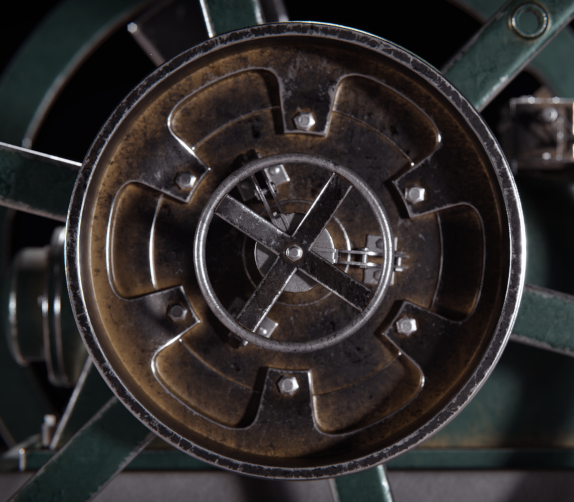
\includegraphics[height=4cm]{images/ex_photoreal}
		\caption{Photorealistic.}\label{ex_photoreal}
	\end{subfigure}
	\begin{subfigure}[b]{0.3\textwidth}
		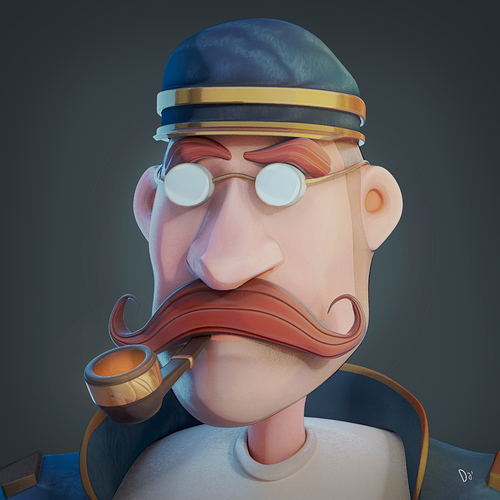
\includegraphics[height=4cm]{images/ex_toon1}
		\caption{Stylised.}\label{ex_toon1}
	\end{subfigure}
	\begin{subfigure}[b]{0.3\textwidth}
		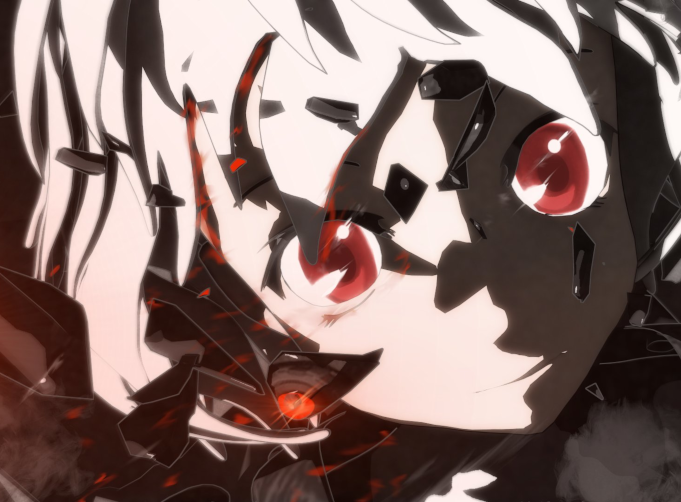
\includegraphics[height=4cm]{images/ex_toon2}
		\caption{Cel.}\label{ex_toon2}
	\end{subfigure}
	\caption{Cycles renderings.}
\end{figure}

The Freestyle\footnote{\url{http://freestyle.sourceforge.net}} edge-and-line-based NPR engine has shipped with Blender as of version 2.67. This engine allows for a wider range of technical and sketchy styles. However, a limitation of Freestyle is the inability to place strokes on faces, which leaves many NPR shading styles such as stippling out of reach. This greatly limits the ability of Freestyle to effectively communicate surface details through traditional techniques.

\begin{figure}[h]
	\centering
	\begin{subfigure}[b]{0.3\textwidth}
		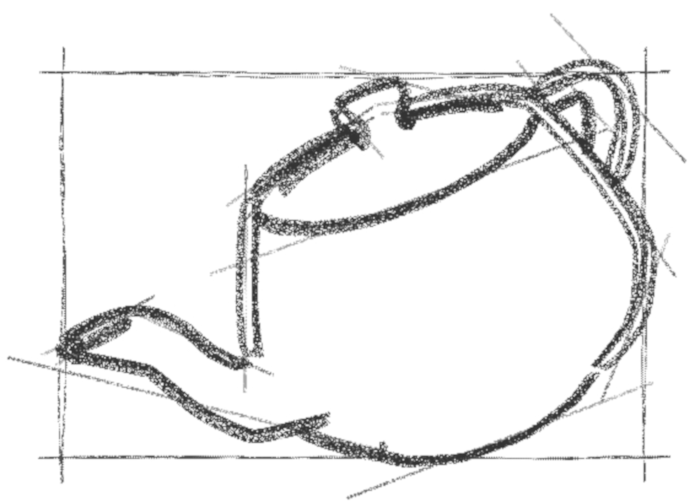
\includegraphics[height=3.25cm]{images/ex_sketchy1}
		\caption{Sketchy.}\label{ex_sketchy1}
	\end{subfigure}
	\begin{subfigure}[b]{0.3\textwidth}
		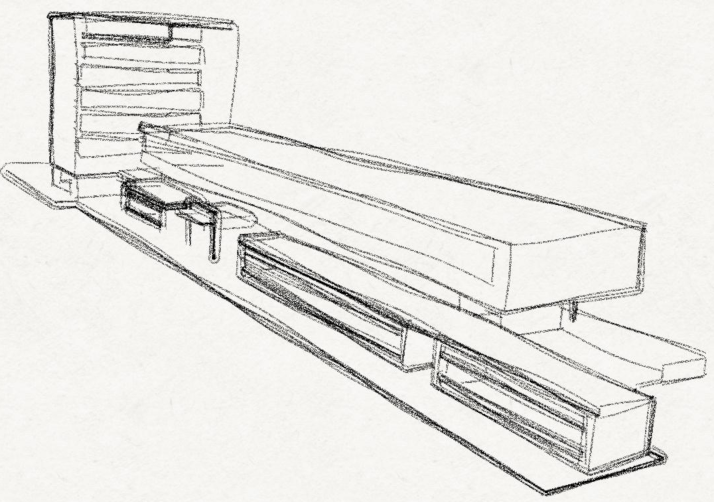
\includegraphics[height=3.25cm]{images/ex_sketchy2}
		\caption{Sketchy.}\label{ex_sketchy2}
	\end{subfigure}
	\begin{subfigure}[b]{0.3\textwidth}
		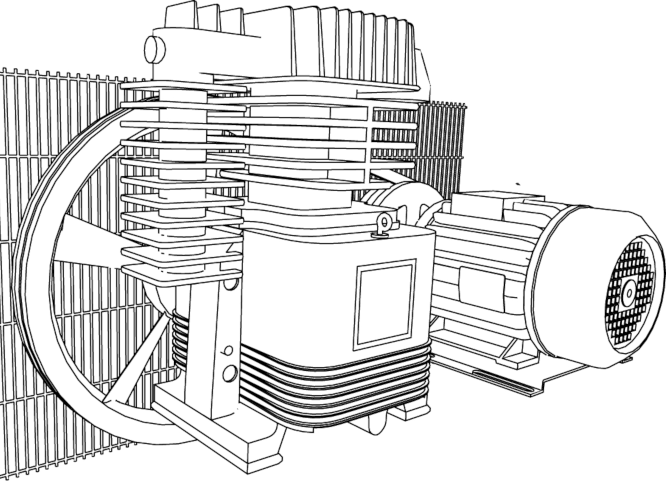
\includegraphics[height=3.25cm]{images/ex_line}
		\caption{Line.}\label{ex_line}
	\end{subfigure}
	\caption{Freestyle renderings.}
\end{figure}

The NPR subfield of Stroke Based Rendering (SBR) presents some interesting techniques to address such shortcommings.
An excellent paper by Aaron Hertzmann (\cite{hertzmann2002}) summarises a selection of SBR approaches to automatically (or semi-automatically) create images by placing discrete strokes, based on some direction from the user.

Hertzmann reports that some techniques - such as Haeberli's painterly algorithm (\cite{haeberli1990}) - have been adpoted into commercial drawing applications, however even today (2018) implementation of technical pen-and-ink styles do not appear to be as accessible.
As such, an opportunity is identified to close this gap.

\section{Problem Definition}

A project is undertaken to extend Blender, by means of developing an add-on, to allow the user to easily produce high-quality renders of traditional, hand-drawn appearance, through application of traditional monochrome drawing techniques.
A user-defined specification will influence the output, allowing the user to choose subtle or bold styles, as suitable for the application.

Scope of the project is limited to communication of mathematical surfaces. The primary use-case is creation of images for publication in technical papers or lecture notes.

\section{Requirements}

